Generally the technologies used for actuation push the pin out of a socket.
The research of \cite{loconsole_braillecursor_2019} explores the use of passive pins and a magnetic rail that pulls each pin, then drops them in a given position that results in up or down. Figure \ref{fig:magnetic-rail} shows this scheme.
While the reduced energy consumption due to passive components is appealing, this solution has an error rate of at least 5\%, and each row of cells necessitates a large motor.
\begin{figure}
\centering
    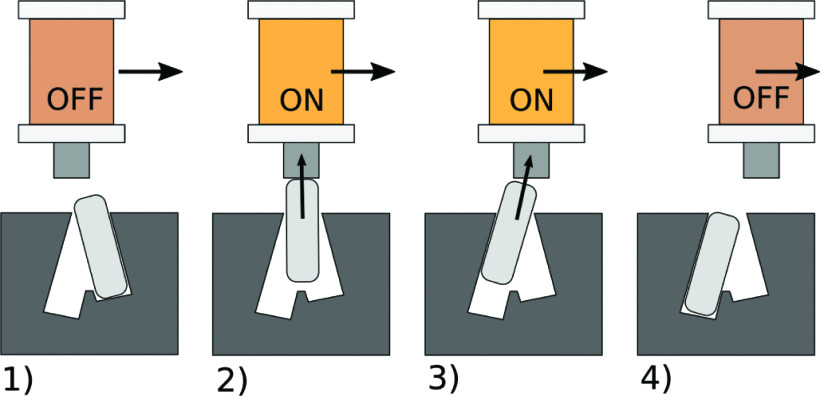
\includegraphics[width=0.6\textwidth]{figures/magnetic-rail.jpg}
\caption{Magnetic rail actuation mechanism. Pins are magnetically pulled from the socket and deposited in either position, having them be on or off (or up and down)}
\label{fig:magnetic-rail}
\end{figure}  

There are some research groups working on braille display system based on dielectric elastomer. Dielectric elastomer is an electroactive polymer that can produce large deformation under the electric field and return to its original size immediately after the electric field being removed. This perfectly satisfies the requirement for making a refreshable braille display. However, this mechanism is strongly dependent on high voltage (HV) supplies and may pose potential dangers to the human body. Although one of the groups suggested using Triboelectric nanogenerators (TENGs) as safer HV supply, we still have to give it up because of the excessive cost and difficulty accessing the same material. 

\begin{figure}\centering
    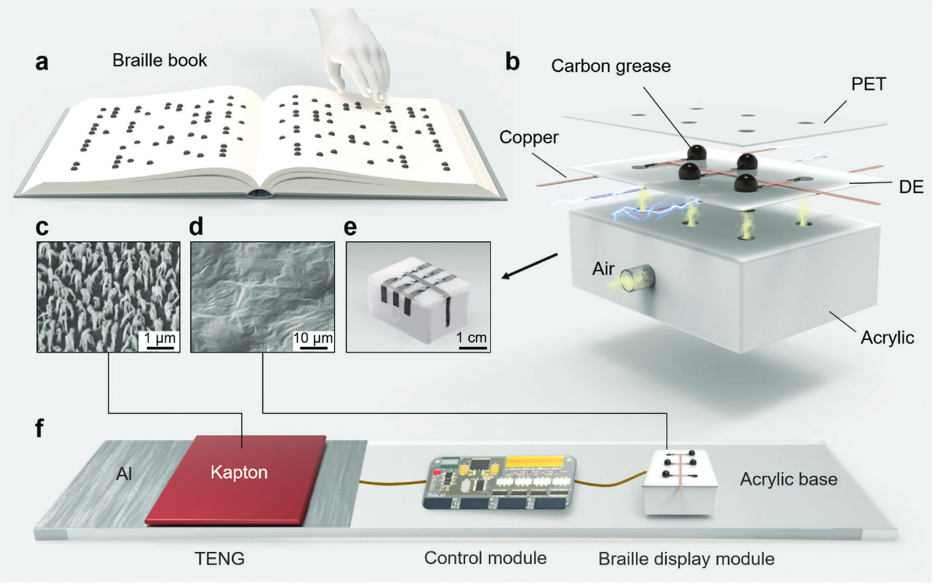
\includegraphics[width=0.6\textwidth]{figures/teng.png}
\caption{}
\label{fig:teng.png}
\end{figure}

Besides, we investigated two mechanisms that rely on heat. Shaped Memory Alloy (SMA), shown in figure \ref{fig:sma}, have the ability to be shaped when cold and return to their predefined original position when heated and thus being a potential solution for actuators in the braille display system.
\begin{figure}\centering
    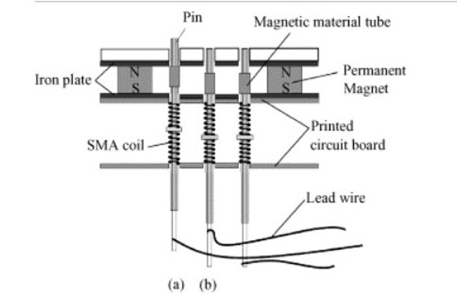
\includegraphics[width=0.6\textwidth]{figures/sma-coil.png}
    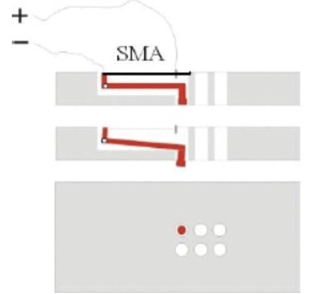
\includegraphics[height=5cm]{figures/sma-mechanism.png}
\caption{}
\label{fig:sma}
\end{figure}

Paraffin wax, shown in figure \ref{fig:paraffin}, can also act as the actuators. When paraffin wax is heated, it expands. The system utilizes the air pressure caused by this expansion to push a mebrane diaphragm up to generate the dots. Both solutions are cheap and the wax based one is especially innovative. However, we did not go with them as they shared a risk of burning the users with the high working temperature and the long cool down period also limits the refreshing rate of the braille display.
\begin{figure} \centering
    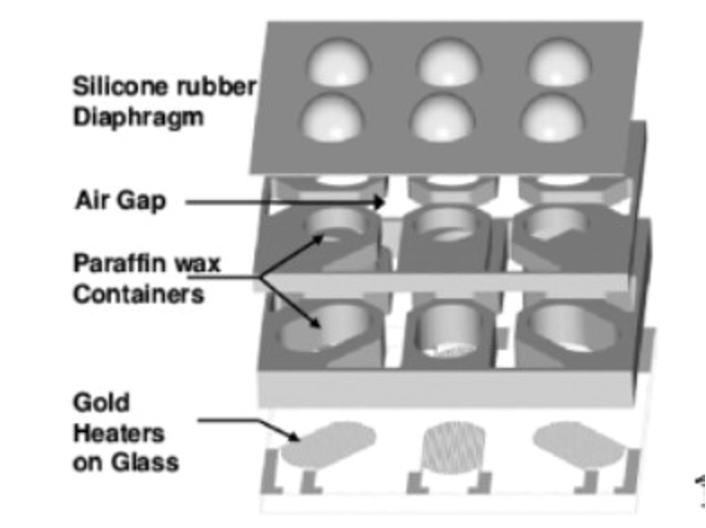
\includegraphics[width=0.6\textwidth]{figures/paraffin.png}
\caption{}
\label{fig:paraffin}
\end{figure}
